\documentclass{beamer}
\usetheme{CambridgeUS}
\usepackage{listings}
\usepackage{blkarray}
\usepackage{listings}
\usepackage{subcaption}
\usepackage{url}
\usepackage{tikz}
\usepackage{tkz-euclide} % loads  TikZ and tkz-base
%\usetkzobj{all}
\usetikzlibrary{calc,math}
\usepackage{float}
\renewcommand{\vec}[1]{\mathbf{#1}}
\usepackage[export]{adjustbox}
\usepackage[utf8]{inputenc}
\usepackage{amsmath}
\usepackage{amsfonts}
\usepackage{tikz}
\usepackage{hyperref}
\usepackage{bm}
\usetikzlibrary{automata, positioning}
\providecommand{\pr}[1]{\ensuremath{\Pr\left(#1\right)}}
\providecommand{\mbf}{\mathbf}
\providecommand{\qfunc}[1]{\ensuremath{Q\left(#1\right)}}
\providecommand{\sbrak}[1]{\ensuremath{{}\left[#1\right]}}
\providecommand{\lsbrak}[1]{\ensuremath{{}\left[#1\right.}}
\providecommand{\rsbrak}[1]{\ensuremath{{}\left.#1\right]}}
\providecommand{\brak}[1]{\ensuremath{\left(#1\right)}}
\providecommand{\lbrak}[1]{\ensuremath{\left(#1\right.}}
\providecommand{\rbrak}[1]{\ensuremath{\left.#1\right)}}
\providecommand{\cbrak}[1]{\ensuremath{\left\{#1\right\}}}
\providecommand{\lcbrak}[1]{\ensuremath{\left\{#1\right.}}
\providecommand{\rcbrak}[1]{\ensuremath{\left.#1\right\}}}
\providecommand{\abs}[1]{\vert#1\vert}

\newcounter{saveenumi}
\newcommand{\seti}{\setcounter{saveenumi}{\value{enumi}}}
\newcommand{\conti}{\setcounter{enumi}{\value{saveenumi}}}
\usepackage{amsmath}
\setbeamertemplate{caption}[numbered]{}

\title{AI1110 Assignment 11}
\author{SADINENI ABHINAY-CS21BTECH11055}
\date{\today}
\logo{\large \LaTeX{}}
\begin{document}
	
	\begin{frame}
		\titlepage
	\end{frame}

\begin{frame}{Outline}
  \tableofcontents
\end{frame}

\section{Abstract}
	\begin{frame}{Abstract}
		\begin{itemize}
			\item 	This document contains the solution to Question of Chapter 8  in the Papoulis Textbook.
		\end{itemize}
	\end{frame}
	
	\section{Question}
	\begin{frame}
	\begin{block}{Ex 8.18}
	The random varible $x_i$ are i.i.d and $\mathcal{N}\brak{0,\sigma}$ We observe that $x_1^2+x_2^2+....x_{10} ^{2}=4$ .Find the 0.95 confidence intervel of $\sigma$.  
	\end{block}
	\end{frame}
	\section{Theory}
	\begin{frame}{Theory}
	\begin{block}{confindence interval}
	The 95\% confidence interval is a range of values that you can be 95\% certain contains the true mean of the population.
	\end{block}
	\begin{block}{chi squared distribution}
	the chi-squared distribution (also chi-square distribution) with k degrees of freedom is the distribution of a sum of the squares of k independent standard normal random variables.
	\end{block}
	\end{frame}
	\section{Solution}
	\begin{frame}{Solution}
	The RVx $x_i/\sigma$ are $\mathcal{N}\brak{0,1}$ hence,the sum $z=\brak{x_1^2+x_2^2+....x_{10} ^{2}}/\sigma^{2}$ has a $\chi^{2} \brak{10}$ This yeilds:
	\begin{align}
	\pr{\chi_{0.025}^{2}\brak{10} < z < \chi_{0.975}^{2}\brak{10} }=0.95  \\
	\chi_{0.025}^{2}\brak{10}=3.25 ,\chi_{0.975}^{2}\brak{10}=20.48 \\
	3.25<\frac{4}{\sigma^2}<20.48 \\
	0.442< \sigma <1.109
	\end{align}
 	\end{frame}
 	\begin{frame}{Output of Code}
 	\begin{figure}[!ht]
		\centering
			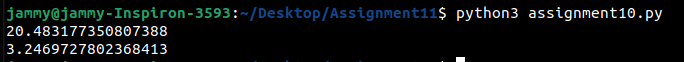
\includegraphics[width=\textwidth,height=5.5cm,keepaspectratio]{figs/output.png}
		\caption{chi square critical values}
		\label{Fig 0:}
	\end{figure}
 	\end{frame}

\end{document}
